\subsubsection{Login}

\paragraph{Anonymous Login}
\begin{figure}[H]
    \centering
    \begin{subfigure}{0.60\linewidth}
        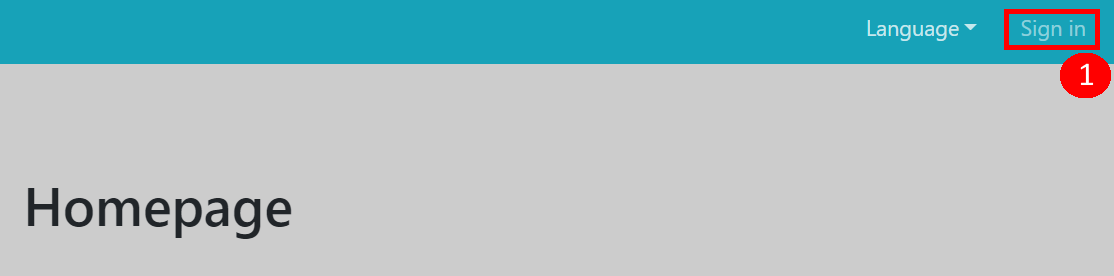
\includegraphics[width=\linewidth]{/userManual/login/mainpage}
       	\caption{}
		\label{fig:annoMainPage}	
    \end{subfigure}
    \begin{subfigure}{0.60\linewidth}
        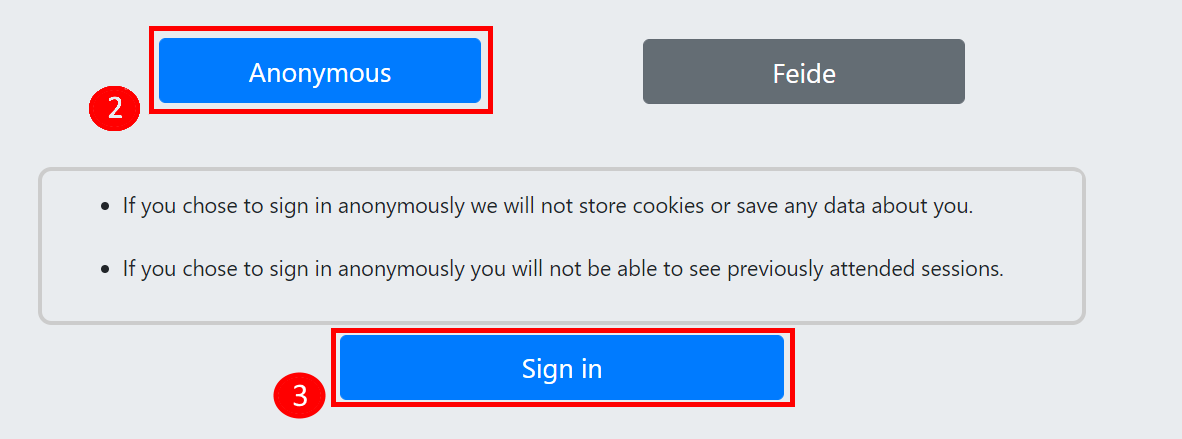
\includegraphics[width=\linewidth]{/userManual/login/annoLogin}
      	\caption{}
		\label{fig:annoLogin}	
    \end{subfigure}
    \begin{subfigure}{0.60\linewidth}
    	
\includegraphics[width=\linewidth]{/userManual/login/annoResult}
    	\caption{}
    	\label{fig:annoResult}	
    \end{subfigure}
\end{figure}

\begin{userManualItemlist}
	\item[Step I.] Click the Sign in button (1). (Figure: \ref{fig:annoMainPage})
	\item[Step II.] Click the button (2) labeled “Anonymous”. (Figure: \ref{fig:annoLogin})
	\item[Step III.] Click the button (3) labeled “Sign in” to anonymously log in to the page. (Figure: \ref{fig:annoLogin})
	\item[Step IV.] If the login was successful, the navigation bar displays a random animal name. (Figure: \ref{fig:annoResult})
\end{userManualItemlist}

\paragraph{Feide Login}
\begin{figure}[H]
    \centering
    \begin{subfigure}{0.60\linewidth}
        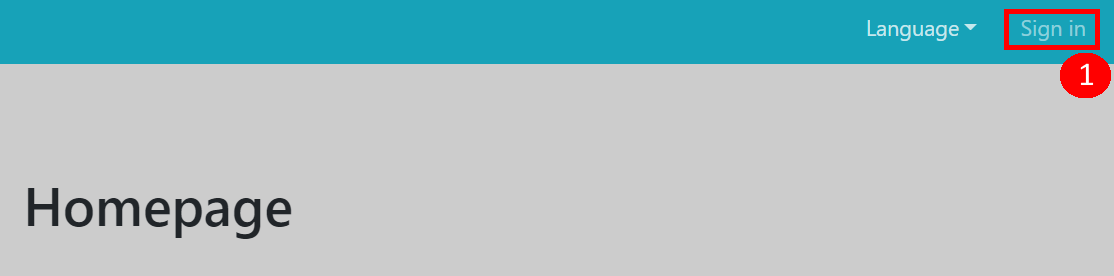
\includegraphics[width=\linewidth]{/userManual/login/mainpage}
       	\caption{}
		\label{fig:feideMainPage}	
    \end{subfigure}
    \begin{subfigure}{0.60\linewidth}
        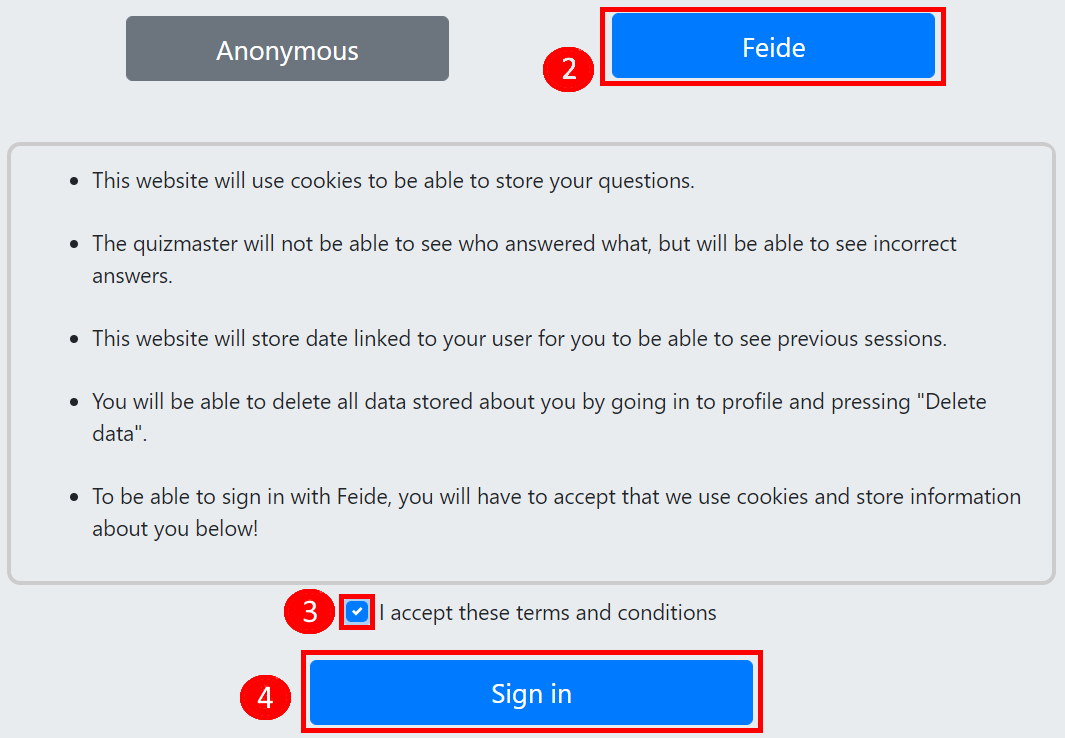
\includegraphics[width=\linewidth]{/userManual/login/feideLogin}
      	\caption{}
		\label{fig:feideLogin}	
    \end{subfigure}
     \begin{subfigure}{0.60\linewidth}
        
\includegraphics[width=\linewidth]{/userManual/login/feideResult}
      	\caption{}
		\label{fig:feideResult}	
    \end{subfigure}
\end{figure}

\begin{userManualItemlist}
	\item[Step I.] Click the Sign in button (1). (Figure: \ref{fig:feideMainPage})
	\item[Step II.] Click the button (2) labeled “Feide”. (Figure: \ref{fig:feideLogin})
	\item[Step III.] Read through the terms of use!  
	\item[Step IV.] Click the radio button (3) (Figure: \ref{fig:feideLogin})
	\item[Step V.] Click the button (4) labeled “Sign in”. (Figure: \ref{fig:feideLogin}) 
	\item[Step VI.] Follow the instructions given and log in to your Feide account.
	\item[Step VII.] If the login was successful, the navigation bar displays your Feide username. (Figure: \ref{fig:feideResult})
\end{userManualItemlist}